\documentclass[11pt, oneside]{article} 
\usepackage{geometry}
\geometry{letterpaper} 
\usepackage{graphicx}
	
\usepackage{amssymb}
\usepackage{amsmath}
\usepackage{parskip}
\usepackage{color}
\usepackage{hyperref}

\graphicspath{{/Users/telliott_admin/Github/Tex/png/}}
% \begin{center} 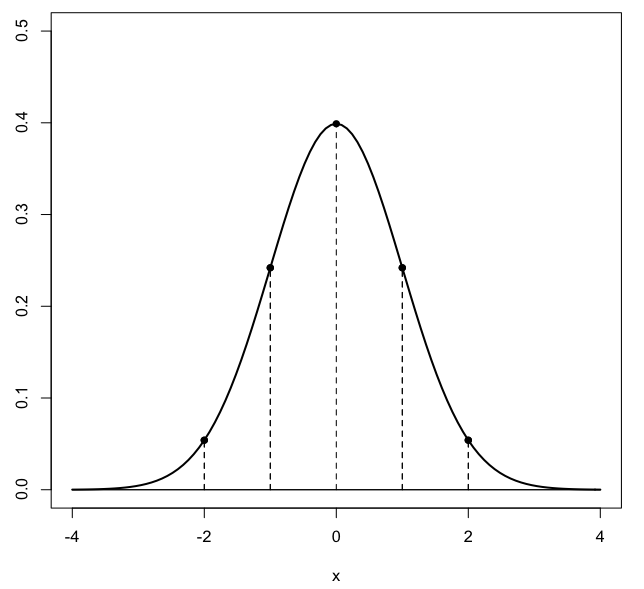
\includegraphics [scale=0.4] {gauss3.png} \end{center}

\title{Rational numbers}
\date{}

\begin{document}
\maketitle
\Large
The integers are great, they give us an infinite supply of numbers.

However, there is a problem with division.  For

\[ p \in \mathbb{N}, \ \ q \in \mathbb{Z} \]

very often the result of $p  \div q$ is not contained in $\mathbb{N}$ or even in $\mathbb{Z}$. We say these sets are not \emph{closed} under division.

For example $3 \div 2 =$ ?

So, we just leave the result as 
\[ \frac{p}{q} = \frac{3}{2} \]

where $p/q$ is in "lowest terms", i.e. they have no common factor other than $1$.  Of course if $p$ is a factor of $q$ or $q$ is a factor of $p$, then we can divide both top and bottom by whichever is smaller (to yield an integer in the case where $q < p$).

$q$ must not be zero because division by zero is not defined.  We \emph{could} choose to allow division by zero, but would quickly run into logical contradictions.

\subsection*{interpolation}
Now, consider two rational numbers, not equal.  Let
\[ s = \frac{p_1}{q_1} \ \ \ t = \frac{p_2}{q_2} \]

Suppose $s < t$.

The \emph{average} of these two rational numbers is:
\[ r = \frac{1}{2} \ [ \ s + t \ ] \]

Then
\[ 2r = s + t \]
\[ 2r - 2s = t - s \]
We have that $s < t$, so $t - s > 0$ and then
\[ r - s > 0 \]
\[ r  > s \]
A similar argument will show that
\[ r < t \]
so
\[ s < r < t \]
$\square$

Thus, one can always find a new rational number that lies between two known rational numbers.

\subsection*{decimal representation}

Every rational number can be represented as a decimal, using the method called long division.

Consider $1/2$
\[ 2 \overline{)1.000} \]

We say that $2$ does not \emph{go into} $1$, since $2 > 1$, so we have the first part of our result as $0$, followed by a decimal point.  But $2$ does go into $10$ exactly $5$ times, giving $0.5$.  The remainder is zero and so the division process terminates.

Consider $1/8$.
\[ 8 \overline{)1.000} \]
$\circ$  $8$ goes into $10$ once, leaving $2$ as remainder

$\circ$  $8$ goes into $20$ twice, leaving $4$.  

$\circ$  $8$ goes into $40$ exactly $5$ times with no remainder.

The result is $0.125$.

The other possibility is that in going through the process a remainder comes up that has been seen previously.  If this happens then the sequence will repeat forever.

If we don't terminate with zero, then this must eventually happen, because there are only as many as $q$ possible remainders.

Thus, for example
\[ 1/7 = 0.142857142857 \dots \]

which contains $142857$, repeating.

\subsection*{decimals to fractions}

Conversely, every repeating decimal can be represented as a rational number.  For example

\begin{verbatim}
      1 x r =      0.142857142857...
1000000 x r = 142857.142857...
 999999 x r = 142857
\end{verbatim}

\[ r = \frac{142857}{999999} = \frac{1}{7} \]
since $7 \times 142857$ equals $999999$ exactly.

You can do this trick with 

\begin{verbatim}
     r = 0.333
10 x r = 3.33
 9 x r = 3
\end{verbatim}

\[ r = \frac{3}{9} = \frac{1}{3} \]

or even

\begin{verbatim}
     r = 0.4999
10 x r = 4.999
 9 x r = 4.5
\end{verbatim}

\[ r = \frac{4.5}{9} = \frac{1}{2} \]

and

\begin{verbatim}
     r = 0.9999
10 x r = 9.999
 9 x r = 9
\end{verbatim}

\[ r = \frac{9}{9} = 1 \]

This is one of the subtleties of numbers.  In what sense can we say that 
\[ 0.5 = 0.4999 \dots \]
\[ 1 = 0.9999 \dots \]

Most everyone is OK with the example $1/3 = 0.3333 \dots$ but some may be uneasy with the other two.

Ultimately, we justify the result as defined by evaluation of a limit.  

Consider $0.9999$.  If $n$ is the number of places in the result, then as $n \rightarrow \infty$ the number being shown approaches $1$ as its limit.  We'll come back to this after considering the real numbers.

\subsection*{ordering}
For two rational numbers $a$ and $b$ there are only three cases:  either $a=b$, $a < b$ or $b < a$.

\[ \frac{p}{q} < \frac{s}{t} \ \iff \ pt < qs \]

$p/q$ is less than $s/t$ if and only if $pt < qs$.  Ordering of the integers guarantees ordering of the rational numbers.

Note:  we used the property of the integers that if
\[ a < b \]
then for $c > 0$
\[ ca < cb \]

\subsection*{intervals}
We denote the numbers greater than $u$ and less than $v$ as lying in the interval $(u,v)$.  With parentheses, the interval described is \emph{open}, it does not include the boundary values.

To describe a \emph{closed} interval, write $[u,v]$.  This interval includes all the values in the first one, plus it also includes $u$ and $v$.

Because of the density property described below, any interval such as
\[ I = [0,1] \]
contains an \emph{infinite} quantity of rational numbers.

\subsection*{density}
Consider the set of all points
\[ x = \frac{p}{10^n} \]
for all natural numbers $n$ and integers $p$.

It is clear that simply by increasing the value of $n$, we can construct a set of equally spaced rational numbers as tightly clustered as we wish.

The rational numbers are said to be \emph{dense} on the number line.  

The method for computing the average of two rational numbers could be used to achieve the same thing.  The result is:

\subsection*{theorem}

$\bullet$  Between \emph{any} two rational numbers it is always possible to find another rational number.  

We might describe this situation by writing that
\[ \forall \ u,v \in \mathbb{Q} \ \exists \ w \in \mathbb{Q} \ | \ w \in (u,v) \]
That's a mouthful!

$\circ$ \ the symbol $\forall$ means "for every" or "for all".

$\circ$ \ the symbol $\exists$ means "there is" or "there exists".

$\circ$ \ the symbol $|$ means "such that".

For every open interval whose bounds are rational numbers, there exists another rational number between $u$ and $v$.


\end{document}
